\documentclass[11pt]{article}
\usepackage{booktabs}
\usepackage{natbib}
\usepackage{fullpage}
\usepackage{fancyhdr}

\usepackage{amsmath}
\usepackage{amssymb}
\usepackage{url}

\usepackage{listings}
\usepackage{color}
\lstset{%
        basicstyle=\footnotesize\ttfamily,
        showspaces=false,
        showstringspaces=false,
        tabsize=2,
        breaklines=false,
        breakatwhitespace=true,
        identifierstyle=\ttfamily,
        keywordstyle=\color[rgb]{0,0,1},
        commentstyle=\color[rgb]{0.133,0.545,0.133},
        stringstyle=\color[rgb]{0.627,0.126,0.941},
    }

\usepackage{graphicx}

% header
\fancyhead{}
\fancyfoot{}
\fancyfoot[C]{\thepage}
\fancyhead[R]{Daniel Foreman-Mackey}
\fancyhead[L]{Statistical Natural Language Processing --- Homework 4}
\pagestyle{fancy}
\setlength{\headsep}{10pt}
\setlength{\headheight}{20pt}

% shortcuts
\newcommand{\Eq}[1]{Equation (\ref{eq:#1})}
\newcommand{\eq}[1]{Equation (\ref{eq:#1})}
\newcommand{\eqlabel}[1]{\label{eq:#1}}
\newcommand{\Fig}[1]{Figure~\ref{fig:#1}}
\newcommand{\fig}[1]{Figure~\ref{fig:#1}}
\newcommand{\figlabel}[1]{\label{fig:#1}}

\newcommand{\etal}{\emph{et al.}}

\newcommand{\pr}[1]{\ensuremath{p\left (#1 \right )}}
\newcommand{\lk}[1]{\ensuremath{\mathcal{L} \left ( #1 \right )}}
\newcommand{\bvec}[1]{\ensuremath{\boldsymbol{#1}}}
\newcommand{\dd}{\ensuremath{\, \mathrm{d}}}
\newcommand{\normal}[2]{\ensuremath{\mathcal{N} \left ( #1; #2 \right ) }}
\newcommand{\T}{^\mathrm{T}}

\newcommand{\data}{\mathcal{D}}
\newcommand{\code}[1]{{\sffamily #1}}
\DeclareMathOperator*{\argmax}{arg\,max}


\begin{document}

I implemented this assignment in pure Python (using extensive use of NumPy for
vectorized operations) and, as you'll see below, I was able to scale the
training to about 250k training sentences.
To go much further than that, further optimizations would be necessary but
this level seemed acceptable for this context.
All of the code that I used for this assignment and the source code for this
document is available on GitHub at \url{https://github.com/dfm/nlp}.

\section{Introduction}

The problem that we're trying to solve in this assignment is word alignment:
given two sentences---one in French and one in English---what is the most
probable set of correspondences between the words.
More concretely, the mathematical quantity of interest is
\begin{eqnarray}\eqlabel{prob}
    p (\bvec{f},\,\bvec{a}\,|\,\bvec{e})\quad,
\end{eqnarray}
the joint probability of a French sentence $\bvec{f}$ (with $m$ words) and
``alignment vector'' $\bvec{a}$ given the English sentence $\bvec{e}$ (with
$l$ words).
In particular, the test that we will implement is based on the maximum
a posteriori alignment $\hat{\bvec{a}}$
\begin{eqnarray}
\hat{\bvec{a}} &=& \argmax_a p (\bvec{f},\,\bvec{a}\,|\,\bvec{e}) \quad.
\end{eqnarray}
This quantity is used in machine translation because in that problem, you
would want to train a model for
\begin{eqnarray}
p(\bvec{e}\,|\,\bvec{f}) &\propto&
    p(\bvec{e})\,p(\bvec{f}\,|\,\bvec{e}) \nonumber\\
    &=& p(\bvec{e})\,
        \sum_a p (\bvec{f},\,\bvec{a}\,|\,\bvec{e}) \quad.
\end{eqnarray}
The \emph{alignment vector} $\bvec{a}$ is a list of integers (of length $m$)
that map positions in $\bvec{f}$ to positions in $\bvec{e}$.
For example, \fig{blue-house} shows two possible alignments between the
sentences $\bvec{e} = blue_1\,house_2$ and
$\bvec{f} = la_1\,maison_2\,bleu_3$.
The left panel shows the alignment associated with the vector
$\bvec{a} = \{-1,\,1,\,2\}$ and the right panel shows $\bvec{a} =
\{-1,\,2,\,1\}$ where $a_i=-1$ indicates the \code{NULL} alignment.

\begin{figure}[htbp]
\begin{center}
    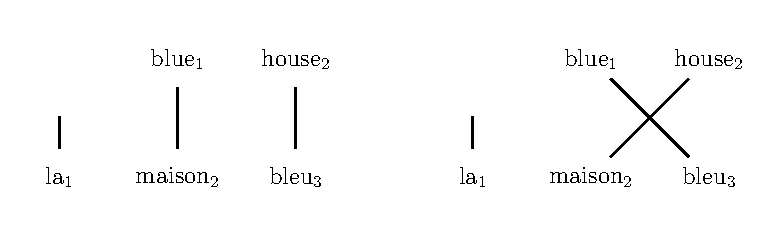
\includegraphics{fig1.pdf}
\end{center}
\caption{%
An example of the possible alignment vectors in a simple sentence pair.
The top line gives the English sentence and the bottom is the French and the
edges indicate the alignment.
\figlabel{blue-house}}
\end{figure}

In this assignment, I'll implement three learning algorithms for \eq{prob}
based on three different sets of independence assumptions.
The first model is based on very simple word-level heuristics and the
following two are the two simplest probabilistic generative models from
\citet{ibm}.

\section{Baseline Model}

The baseline model is a diagonal alignment $\hat{\bvec{a}} = \{a_i =
i,\,\mathrm{for}\,i=1,\,\cdots,\,m\}$.
For comparison, this model achieves a precision of 33.5\%, a recall of 19.8\%
and an AER of 71.2\% on the provided validation set.
We can also run this model on the provided \code{miniTest} dataset and find a
precision and recall of 88.9\% and an AER of 11.1\%.

\section{Heuristic Model}

The first more sophisticated model that we were to implement is a model based
on some sort of word-level heuristics.
I chose to use word co-occurrence rates as the heuristic.
In practice, this means that
\begin{eqnarray}
p(\bvec{f},\,\bvec{a}\,|\,\bvec{e}) &=&
    \prod_{i=1}^m \frac{c(f_i,\,e_{a_i})}{c(f_i)\,c(e_{a_i})} \quad.
\end{eqnarray}
where $c(f_i,\,e_{a_i})$ is the number of times that both $f_i$ and $e_{a_i}$
appear together in a sentence pair and $c(f_i)$ and $c(e_{a_i})$ are the
total number of times that $f_i$ and $e_{a_i}$, respectively, appear in the
training data.
The only complication in this model comes when an unknown French word appears.
I chose to deal with this by falling back on the baseline (diagonal) alignment
for these unknown words.

On the \code{miniTest}, this model gives a precision of 81.8\%, a perfect
recall and an AER of 10\%.
For the validation data, the results (as a function of the number of training
sentence pairs used) are shown in Table~\ref{tab:heuristic} and
\fig{heuristic}.
Given the extreme simplicity and ease of training (even with 500k training
sentences the model trained in less than a minute on my basic MacBook Pro),
the minimum AER of 35.0\% using 500k training examples seems pretty impressive.
It's also interesting to note how drastically the results improve as more data
are used to train.

\begin{table}[htbp]
\begin{center}
\begin{tabular}{c ccc}
\toprule
$N_\mathrm{train}$ & precision [\%] & recall [\%] & AER [\%] \\\midrule
500 & 37.553 & 42.012 & 60.999 \\
1000 & 39.403 & 43.787 & 59.174 \\
5000 & 45.594 & 54.438 & 51.567 \\
10000 & 47.838 & 59.763 & 48.341 \\
100000 & 57.778 & 71.006 & 37.996 \\
500000 & 61.165 & 73.077 & 35.033 \\
\bottomrule
\end{tabular}
\end{center}
\caption{%
The performance the heuristic word-alignment model on the validation dataset
as a function of the number $N_\mathrm{train}$ of training sentence pairs used.
\label{tab:heuristic}}
\end{table}

\begin{figure}[htbp]
\begin{center}
    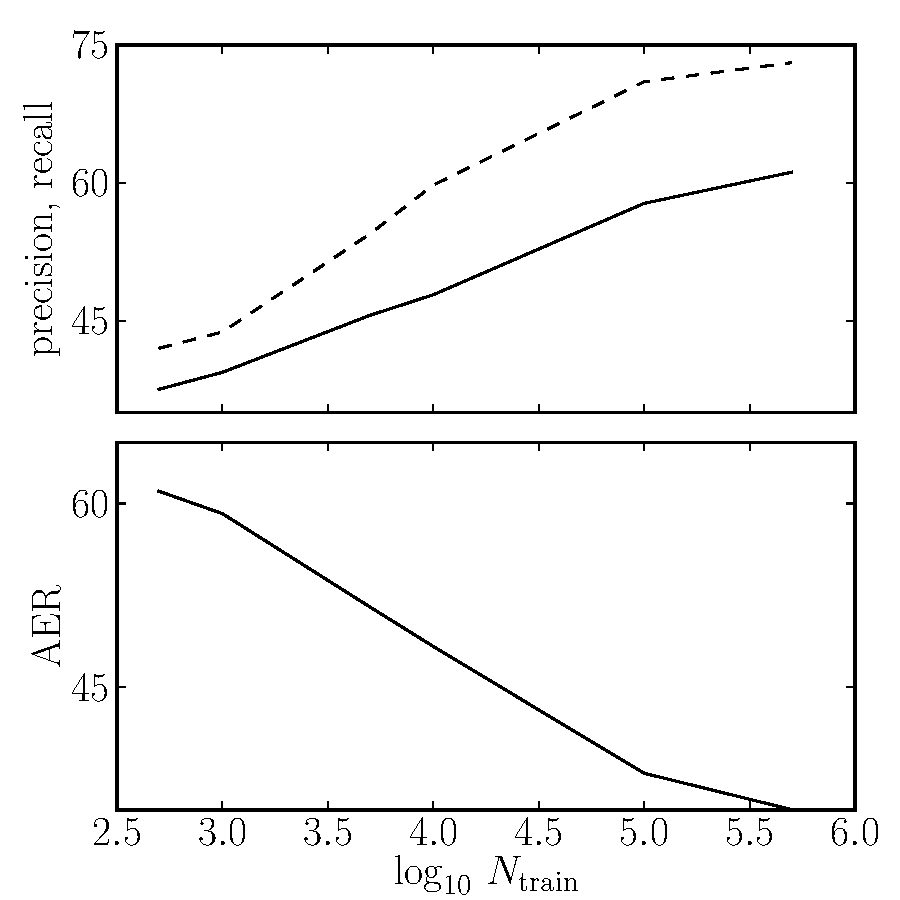
\includegraphics[width=0.5\textwidth]{heuristic.pdf}
\end{center}
\caption{%
The performance the heuristic word-alignment model on the validation dataset
as a function of the number $N_\mathrm{train}$ of training sentence pairs used.
The top panel shows the precision (solid line) and the recall (dashed line)
and the bottom panel shows the AER.
\figlabel{heuristic}}
\end{figure}

\section{IBM Model 1}

The next two models that I will consider are the first two models presented by
\citet{ibm}.
Both start from a particular factorization of \eq{prob}
\begin{eqnarray}
p(\bvec{f},\,\bvec{a}\,|\,\bvec{e}) &=&
    p(m\,|\,\bvec{e}) \, \prod_{i=0}^m p(a_i\,|\,m,\,l)\,p(f_i\,|\,e_{a_i})
    \quad.
\end{eqnarray}
Note that this equation is \emph{not} as general as \eq{prob}.
In particular, the main independence assumptions that go into this
factorization are that (a) the alignment probabilities are conditionally
independent given (only) the sentence lengths and (b) the translation
probabilities for each word pair are independent of the other words in the
sentence.
These are clearly brutal assumptions (especially given what we've learned
already in this course) but they do make the problem tractable.
We'll actually go one step further \citep[following][]{ibm} and assume the
prior probability on the French sentence length is a small (irrelevant)
constant $p(m\,|\,\bvec{e}) \equiv \epsilon$.
For \emph{Model 1}, we'll make the further assumption that the alignment
probabilities are uniform across the whole sentence
\begin{eqnarray}
p(a_i\,|\,m,\,l) &=& \frac{1}{1+l} \quad.
\end{eqnarray}
With these assumptions, the probabilistic model that we want to learn is
\begin{eqnarray}
p(\bvec{f},\,\bvec{a}\,|\,\bvec{e}) &=&
    \frac{\epsilon}{1+l}\,\prod_i p(f_i\,|\,e_{a_i}) \quad.
\end{eqnarray}
In practice, I included the \code{NULL} token in each English sentence and
special cased the alignment to that position to have a constant prior
probability $P_\mathrm{NULL}$ of alignment.
I chose to set this to $P_\mathrm{NULL}$ using a not particularly scientific
set of experiments but the results don't seem to be very sensitive to this
value.
Under this model, the parameters $p(f_i\,|\,e_j)$ and
$p(f_i\,|\,\mathrm{NULL})$ can be learned using expectation maximization (EM).
The steps are as follows:
\begin{enumerate}
\item{initialize the parameters uniformly,}
\item{\emph{expectation}: using the current settings of the parameters,
      compute the posterior probabilities
      $p(\bvec{a}\,|\,\bvec{f},\,\bvec{e})$ for each sentence pair,}
\item{\emph{maximization}: find the maximum likelihood values for the
      parameters $p(f_i\,|\,e_j)$ using the estimated posteriors
      from the previous step.}
\end{enumerate}
In practice, this last step simply involves summing the effective
counts---weighted by the posterior probabilities---for each word pair and
normalizing properly.

Running this model on the \code{miniTest} dataset for about 3 iterations of
EM converges quickly leaving only the following error:
\begin{lstlisting}
    [#]   | U
     # [ ]| V
     #    | W
    ------'
     D  F
\end{lstlisting}
The performance of this model on the validation data as a function of training
set size is shown in Table~\ref{tab:model1} and plotted in \fig{model1}.
For each of these experiments, 10 iterations of EM were used.
\Fig{model1-convergence} shows the performance of this model on the validation
data as a function of the number of iterations of EM.
Interestingly, the best predictions are made after only one step of EM despite
the fact that the likelihood of the model is improving on the training data.
This effect is probably due to over-fitting.
The model has a very large number of parameters and no regularization or prior
on them to ensure reasonable values.

\begin{table}[htbp]
\begin{center}
\begin{tabular}{c ccc}
\toprule
$N_\mathrm{train}$ & precision [\%] & recall [\%] & AER [\%] \\\midrule
500 & 35.098 & 35.799 & 64.665 \\
1000 & 38.427 & 41.420 & 60.573 \\
5000 & 52.000 & 55.030 & 46.964 \\
10000 & 55.522 & 58.876 & 43.343 \\
100000 & 60.602 & 63.314 & 38.485 \\
500000 & 64.363 & 67.160 & 34.681 \\
\bottomrule
\end{tabular}
\end{center}
\caption{%
The same as Table~\ref{tab:heuristic} but using \emph{Model 1}.
\label{tab:model1}}
\end{table}

\begin{figure}[htbp]
\begin{center}
    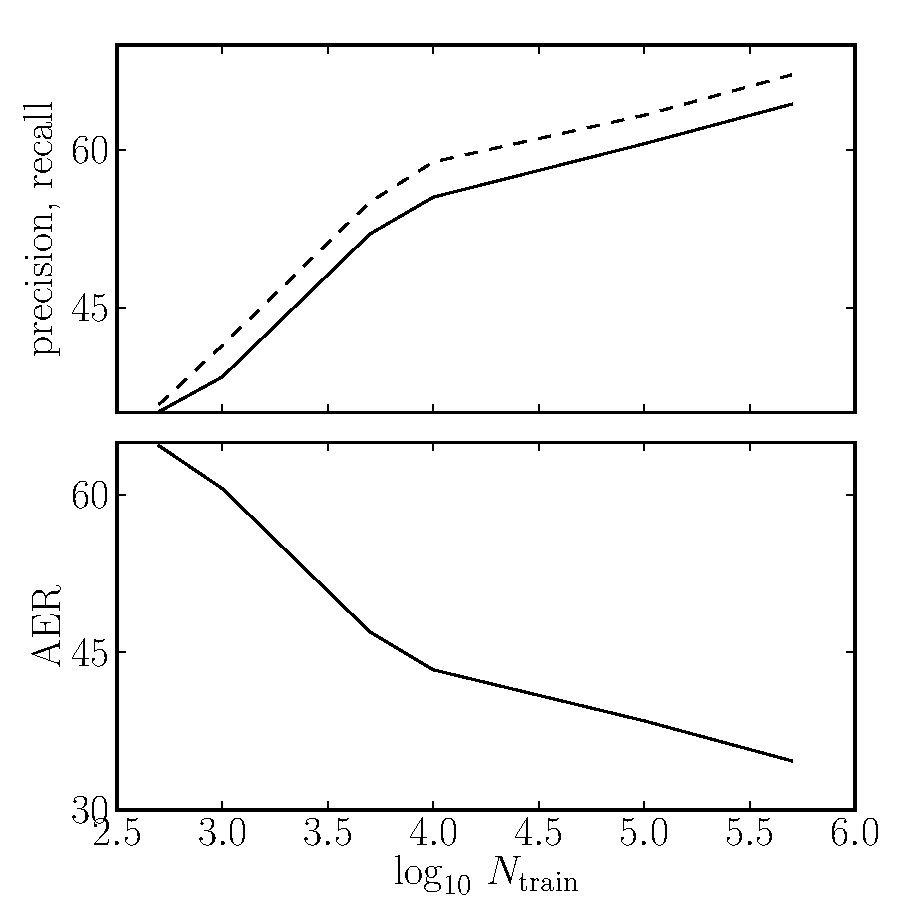
\includegraphics[width=0.5\textwidth]{model1.pdf}
\end{center}
\caption{%
The same as \fig{heuristic} but using \emph{Model 1}.
\figlabel{model1}}
\end{figure}

\begin{figure}[htbp]
\begin{center}
    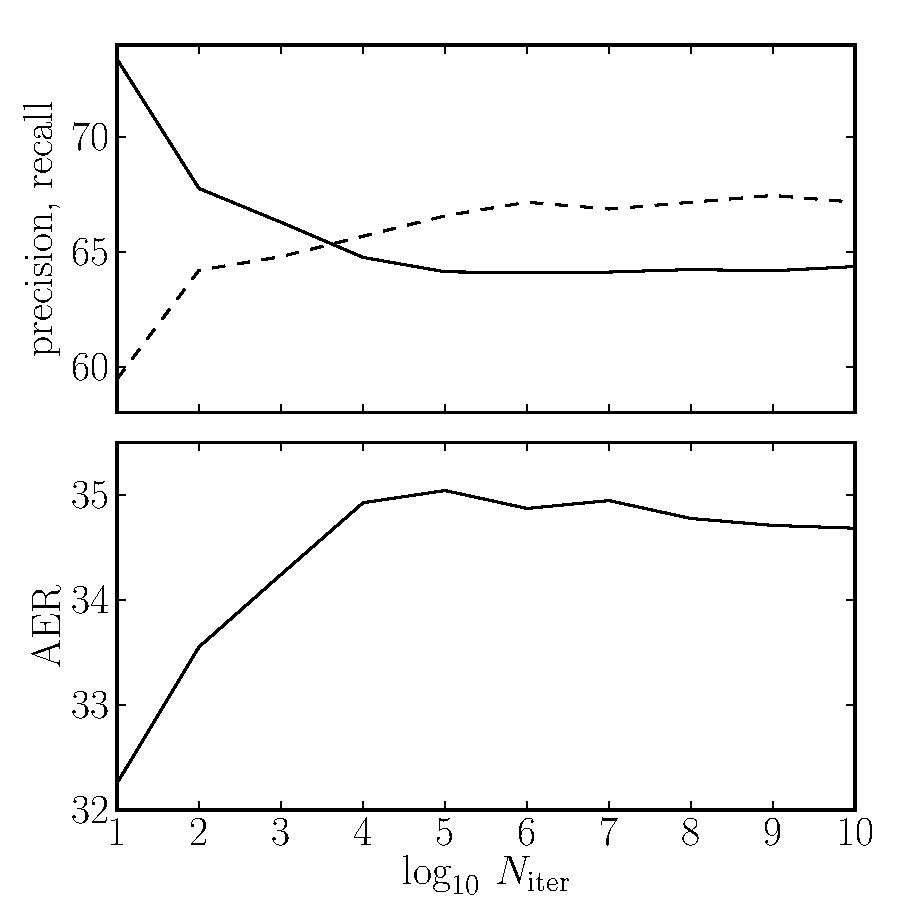
\includegraphics[width=0.5\textwidth]{model1_convergence.pdf}
\end{center}
\caption{%
The performance of \emph{Model 1} (using 500k training sentence pairs) as a
function of the number of EM iterations.
The top panel shows the precision (solid line) and the recall (dashed line)
and the bottom panel shows the AER.
\figlabel{model1-convergence}}
\end{figure}

\section{IBM Model 2}

The second probabilistic model introduces a parametrized alignment probability
function to apply prior linguistic knowledge and, as a result, regularize the
parameters from the previous model.
As suggested in the assignment, I decided to model the alignment probability
using the Laplace distribution
\begin{eqnarray}\eqlabel{model2-prob}
p(a_i\,|\,m,\,l) &\propto& \exp \left ( -\alpha\,\frac{l}{m} \,
                                        \left | i - a_i \right | \right )
        \quad.
\end{eqnarray}
I also tried a Gaussian but the results weren't quite as good so I won't
discuss them much here.
I think that the main problem with the Gaussian is that there isn't enough
support in the wings to allow for larger jumps in alignment (even though these
can happen).
As a result, it might be interesting to try a distribution with heavier tails.

Most of the learning procedure from the previous section carries over to this
model.
The first difference is that the posterior probabilities for $\bvec{a}$ must
be computed including the term from \eq{model2-prob}.
Secondly, the \emph{maximization} step must also include an update to the
parameter $\alpha$.
Since \eq{model2-prob} is the well known Laplace distribution, the maximum
likelihood value for $\alpha$ is simply
\begin{eqnarray}
\frac{1}{\hat{\alpha}} &=& \frac{\displaystyle{\sum_k w_k \, \frac{l_k\,| i-a_i
    |_k}{m_k}}}{\displaystyle{\sum_k w_k}}
\end{eqnarray}
where the sums are over all possibly aligned pairs and $w_k =
p(a_i\,|\,m,\,l)\,p(f_i\,|\,e_{a_i})$.
This update is trivial to compute given the results needed to update the word
translation probabilities.
In all of the following examples, I initialized $\alpha$ as 0.3.

We still have the problem that when we encounter new French words, the
probability function will be zero and any alignment will be rejected.
Once again, I fall back on the alignment only model (which becomes exactly
the baseline diagonal model in this case) and align the word based on just
that.
It seems like it would probably be helpful to include some sort of unknown
word model that compares features of the different words to produce a
probability of alignment.
This would probably work well for English and French where many words have
similarities in both languages.

Running this model on \code{miniTest} gives a near perfect solution (with a
slightly sub-optimal precision because of the final block:
\begin{lstlisting}
    [#]   | U
       [#]| V
        # | W
    ------'
     D  F
\end{lstlisting}
When converged, this model found a maximum likelihood value of $\alpha=6.0$.

The results of this model are also substantially better when tested on the
validation set.
Table~\ref{tab:model2} shows the performance as a function of the number of
training samples and these data are plotted in \fig{model2}.
\Fig{model2-convergence} shows the validation performance as a function of the
number of iterations of EM.
In an earlier test, I found that the validation performance began to get worse
after $\sim 5$ iterations so I decided to stop after 5 for this example.
In fact, the best performance appears after 4 iterations (with an AER of
22.8\%) and then gets worse (AER of 23.0\% after 5 iterations).
This behavior is more consistent with my expectations.
It doesn't converge immediately after one step because of the regularization
and then it converges to a much better solution than \emph{Model 1} (without
over-fitting) because of the model is less flexible in exactly the right
direction.

\paragraph{Remaining errors}
Unfortunately my final model doesn't manage to reach an AER of $<20\%$ on
either the validation set or the test set even when a substantial fraction of
the training sentences are used.
I even tried running with the full set of training examples for a few
iterations of EM (this took quite a while) and found only a marginal
improvement over the 500k sentences.
There are a few reasons why this might happen.
First, this might be due to numerical effects; there are a few places in the
code where I'm using probabilities when I should be using log-probabilities.
This is a pretty silly mistake and it seems a likely cause of
trouble---especially when considering rare words.
Second, there are two tuning parameters that I haven't really discussed at
all: (1) the prior probability on the \code{NULL} alignment and (2) the
initial value of $\alpha$.
I don't think that these should be a problem based on some experimentation.
Furthermore, I think (without proof) that the objective function should be
convex like \emph{Model 1} so the initial values of the parameters shouldn't
matter unless there's a bug in the code.

\begin{table}[htbp]
\begin{center}
\begin{tabular}{c ccc}
\toprule
$N_\mathrm{train}$ & precision [\%] & recall [\%] & AER [\%] \\\midrule
500 & 48.451 & 56.805 & 48.855 \\
1000 & 55.603 & 65.385 & 41.199 \\
5000 & 63.329 & 76.923 & 32.283 \\
10000 & 65.678 & 78.698 & 30.115 \\
100000 & 69.448 & 81.953 & 26.507 \\
200000 & 71.469 & 84.024 & 24.474 \\
500000 & 73.371 & 84.320 & 23.084 \\
\bottomrule
\end{tabular}
\end{center}
\caption{%
The performance IBM Model 2 on the validation dataset
as a function of the number $N_\mathrm{train}$ of training sentence pairs used.
\label{tab:model2}}
\end{table}

\begin{figure}[htbp]
\begin{center}
    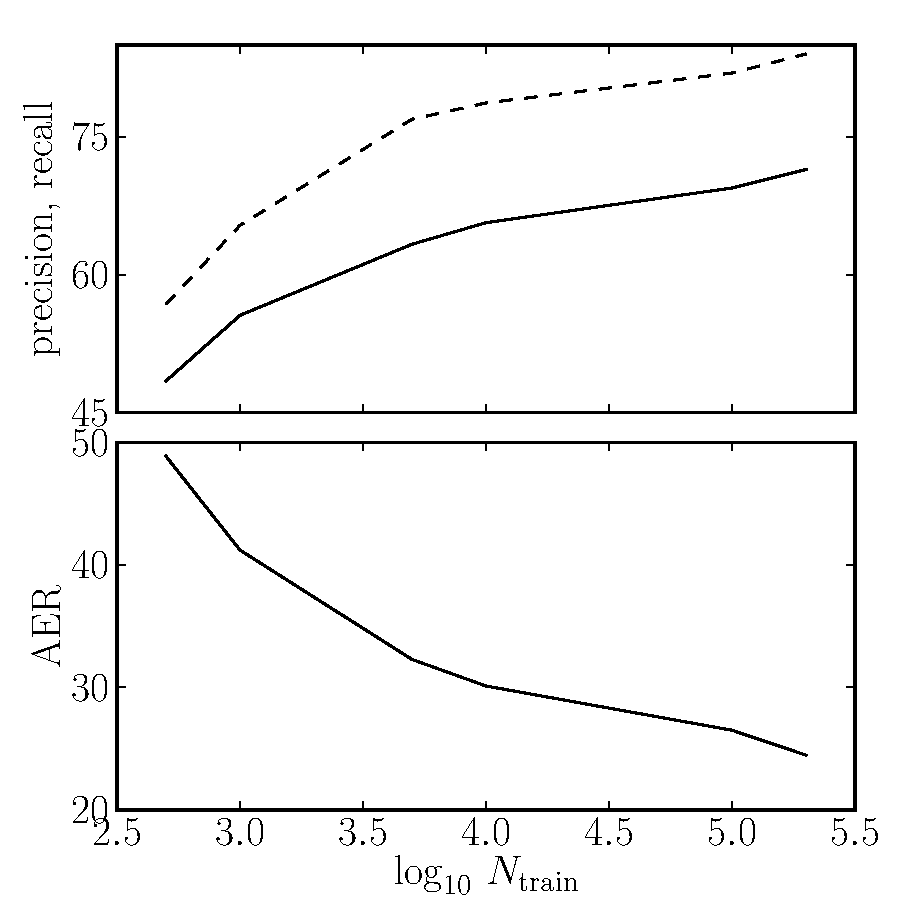
\includegraphics[width=0.5\textwidth]{model2.pdf}
\end{center}
\caption{%
The same as \fig{heuristic} but using \emph{Model 2}.
\figlabel{model2}}
\end{figure}

\begin{figure}[htbp]
\begin{center}
    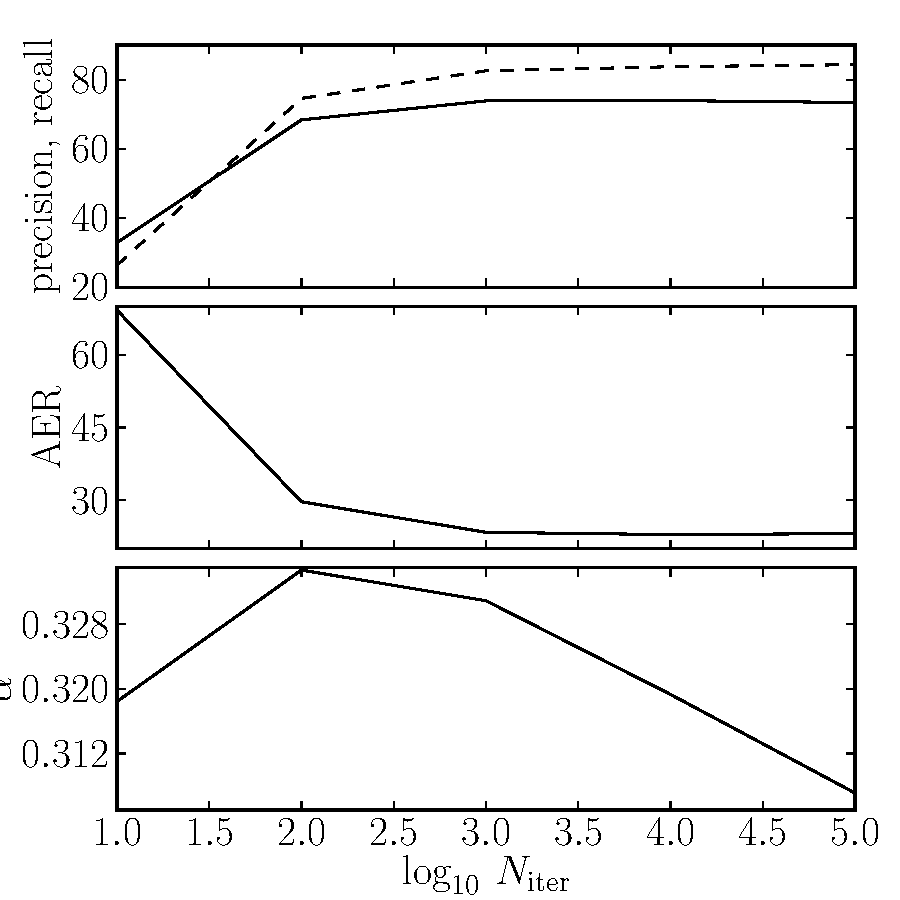
\includegraphics[width=0.5\textwidth]{model2_convergence.pdf}
\end{center}
\caption{%
The same as \fig{model2-convergence} but using \emph{Model 2}.
The bottom panel here shows the value of $\alpha$ at each step.
\figlabel{model2-convergence}}
\end{figure}

\begin{thebibliography}{}\raggedright

\bibitem[Brown \etal(1993)]{ibm}
P.~F.~Brown, S.~A.~Della\ Pietra, V.~J.~Della\ Pietra, \& R.~L.~Mercer (1993)
\textbf{The Mathematics of Statistical Machine Translation: Parameter
        Estimation}, Computational Linguistics, 19, 2

\end{thebibliography}

\end{document}
